\section{Spectra analysis}
The approximate sweet spot for Am and Fe were rough gain of $4$ and bias voltage of $1937$ V. The measurement times are listed in table \ref{tab:measurementstimes}. In this section, the figures for the can and aluminium pipe detectors will be shown side-by-side with the can detector on the left and the aluminium detector on the right.

\begin{table}[hb!]
\begin{tabular}{lll}
\textbf{Detector}    & \textbf{Source} & \textbf{Live time {[}min.{]}} \\ \hline
\multirow{3}{*}{Can} & Fe-55           & 5                          \\
                     & Am-241          & 15                         \\
                     & Bkg             & 45                         \\ \hline
\multirow{3}{*}{Alu} & Fe-55           & 19                         \\
                     & Am-241          & 25                         \\
                     & Bkg             & 30                         \\ \hline
\end{tabular}
\caption{List of measurement times for the different sources and setups.}
\label{tab:measurementstimes}
\end{table}

When the sources are measured, the data files are loaded into histograms which are then converted to cubic basis splines (B-splines) with smoothing of 0.02 for the sources and 0.002 for the background. These are shown as dashed lines in fig. \ref{dig:spectra}. The Am and background spectra are normalized to the Fe spectrum. The splined background is then subtracted from the splined sources and binned into 1024 bits and shown as the full lines in the figure. For the aluminium pipe, the spline procedure does distort the escape peak somewhat.

\begin{figure*}[htb]
  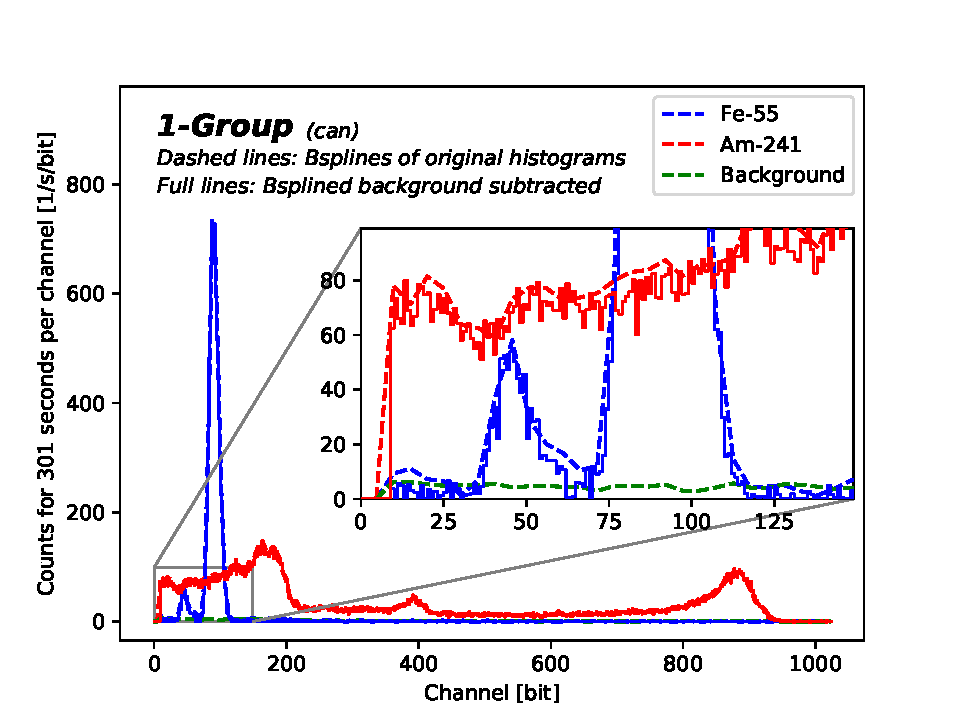
\includegraphics[width=0.49\textwidth,page=1]{graphics/bkgsubtraction.pdf}
  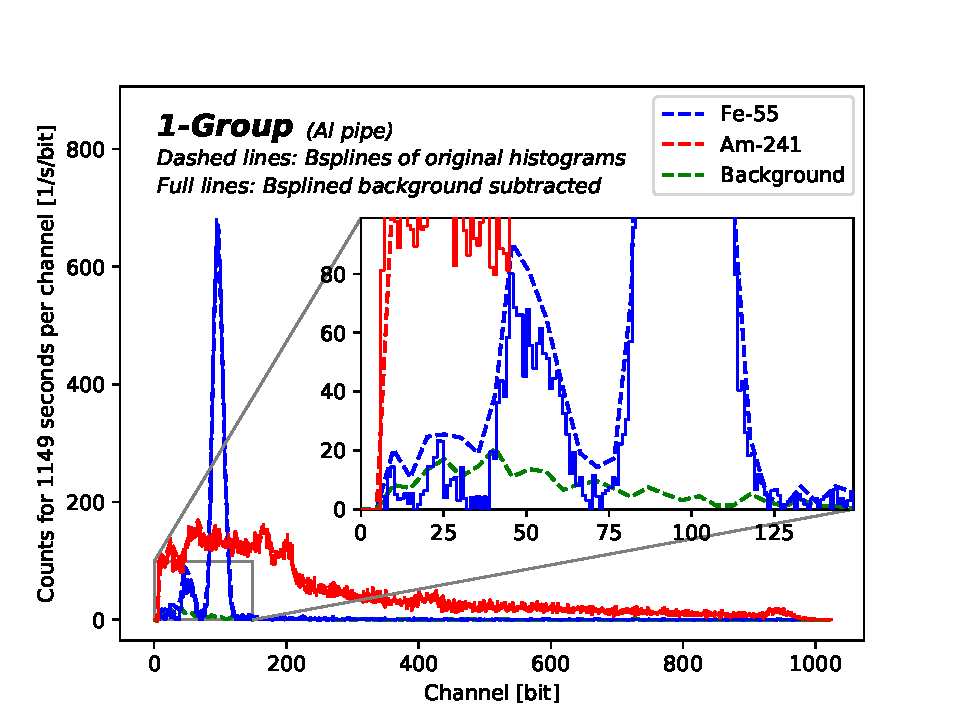
\includegraphics[width=0.49\textwidth,page=1]{graphics/alubkgsubtraction.pdf}
  %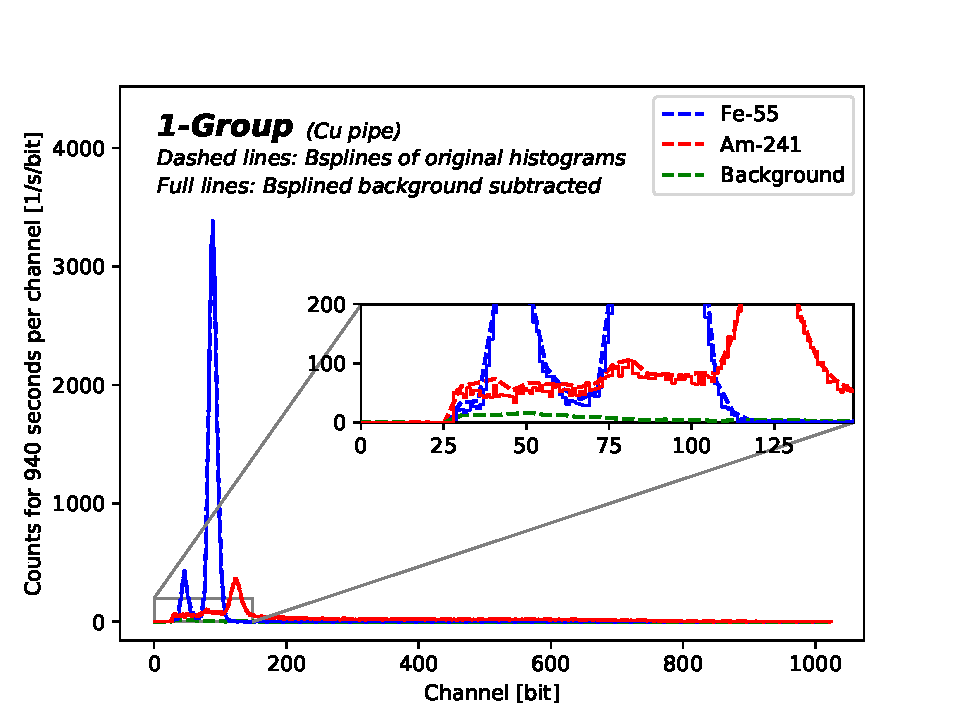
\includegraphics[width=0.32\textwidth,page=1]{graphics/cupbkgsubtraction.pdf}
  \caption{Spectra of Fe and Am as well as background for the can detector and the aluminium pipe. Am and background have been normalized to the Fe spectra. The dashed lines are splines of the original histograms, and the full lines are the splined sources with splined background subtracted. The shown resolution of the splines is intentionally low.}
  \label{fig:spectra}
\end{figure*}

All subsequent figures will only be shown with the background subtracted.

Gaussian fits are then performed on the known Fe and Am peaks. All fits are performed using Chisquare minimization only. Different fit functions are used and detailed in table \ref{tab:fitfuncchannelfits}. Fits are first performed with strict bounds which are then entirely lifted to show stability and for correctness of uncertainties. For the can detector, only bins with values larger than 20 are used for the escape peak and the Am peak. For the Fe double gaussian, the fit spans further in order to reach convergence for the unbounded fit. For the aluminium pipe, the escape peak is badly shaped, possibly due to the spline procedure. Therefore, the fit is performed from the right tail and above the peak until the shape deterioates. For the Fe double gaussian, some of the left side is left out to help convergence of the unbounded fit. For both detectors, the left side of the Am peak is not well modeled by a single gaussian peak, wherefore it is mostly left out from the fit.

For the escape peak fits, a regular gaussian is used. For the Fe peak, the uncorrelated gaussian double gaussian is used. For the Am peak, a regular gaussian is used for the can detector. However, for the aluminium pipe, a 1st order polynomial must be added to ensure convergence.

% \begin{tabular}[c]{@{}l@{}}Uncorrelated\\ double gaussian\end{tabular}
\begin{table*}[htb!]
\begin{tabular}{ll}
\textbf{Name}                 & \textbf{Expression} \\ \hline
Gaussian                      & $\frac{N}{\sqrt{2\pi}\sigma}\exp{\left(-\frac{\left(x-\mu\right)^2}{2\sigma^2}\right)}$                    \\
Uncorrelated double gaussian  & $N\left[r\frac{1}{\sqrt{2\pi}\sigma}\exp{\left(-\frac{\left(x-\mu\right)^2}{2\sigma^2}\right)}+(1-r)\frac{1}{\sqrt{2\pi}\sigma}\exp{\left(-\frac{\left(x-\mu\right)^2}{2\sigma^2}\right)}\right]$                     \\
Gaussian plus 1st order poly. & $\frac{N}{\sqrt{2\pi}\sigma}\exp{\left(-\frac{\left(x-\mu\right)^2}{2\sigma^2}\right)} + b + ax$                   
\end{tabular}
\caption{Expressions for the used fit functions for the gaussian fits. These are regular gaussian functions with a normalization factor. The uncorrelated double gaussian expression is used for fits with overlapping signals, and has less correlated parameters than two regular gaussians. The parameters are the usual gaussian parameters as well as the normalization factor, $N$, the ratio, $r$, and the polynomial factors of the y-intersection, $b$, and slope $a$.}
\label{tab:fitfuncchannelfits}
\end{table*}

\begin{figure*}[htb]
  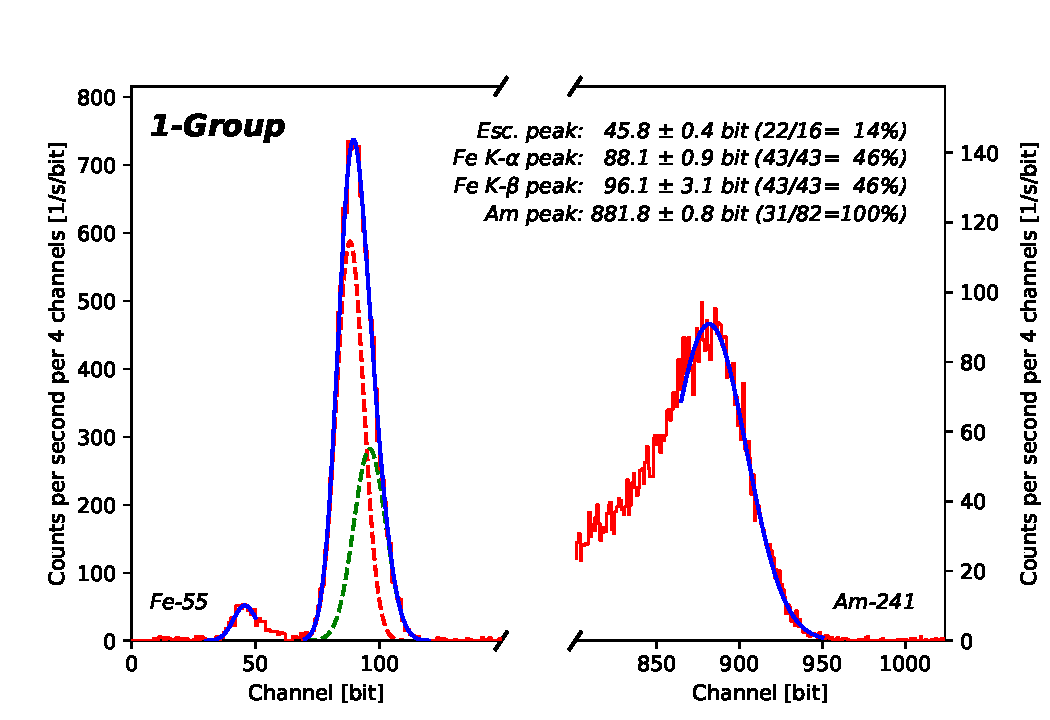
\includegraphics[width=0.49\textwidth,page=1]{graphics/channelfits.pdf}
  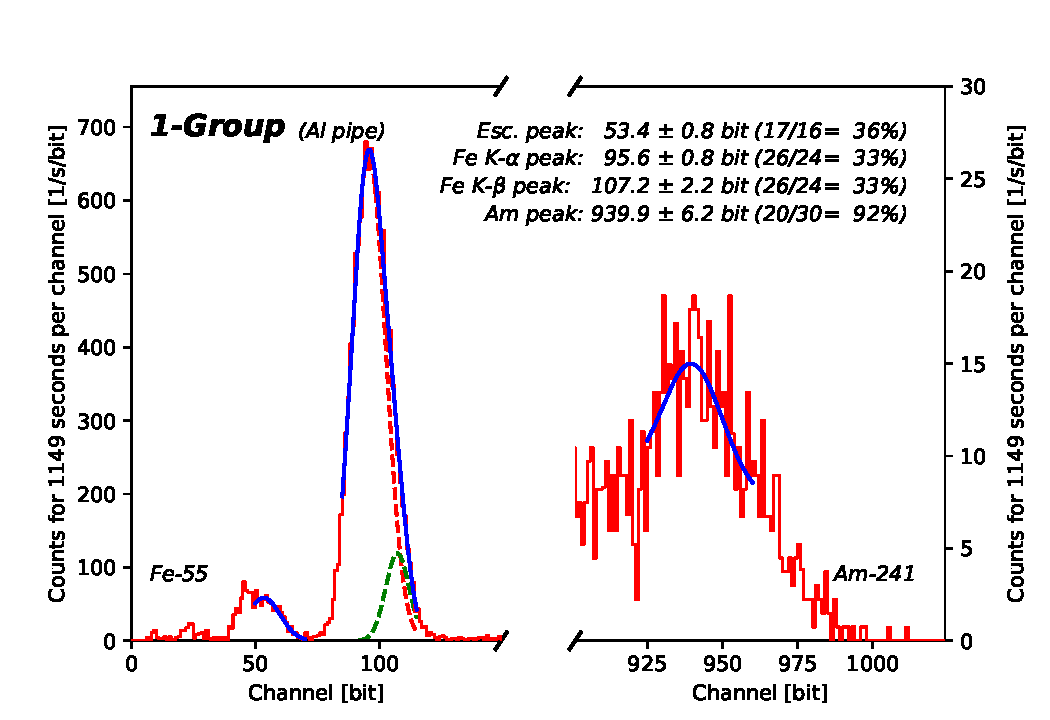
\includegraphics[width=0.49\textwidth,page=1]{graphics/aluchannelfits.pdf}
  \caption{Fits to the four known peaks, the escape peak, the double iron, and the americium. The single gaussians of the double iron peak are shown as dashed lines. The resulting centroids of the fits are shown in the figure along with the Chisquare value, number degrees of freedom, and the Chisquare probability. Note the broken x-axis.}
  \label{fig:channelfits}
\end{figure*}

After extracting the centroids, the four peaks are plotted against their known energies and a 1st order polynomial fit is performed. The result is shown in fig \ref{fig:energychannelcalib}. For the aluminium detector, the low Chisquare value is due to the larger uncertainties coming from the poor gaussian fits, and the y-intersection is not consistent with 0.

\begin{figure*}[htb]
  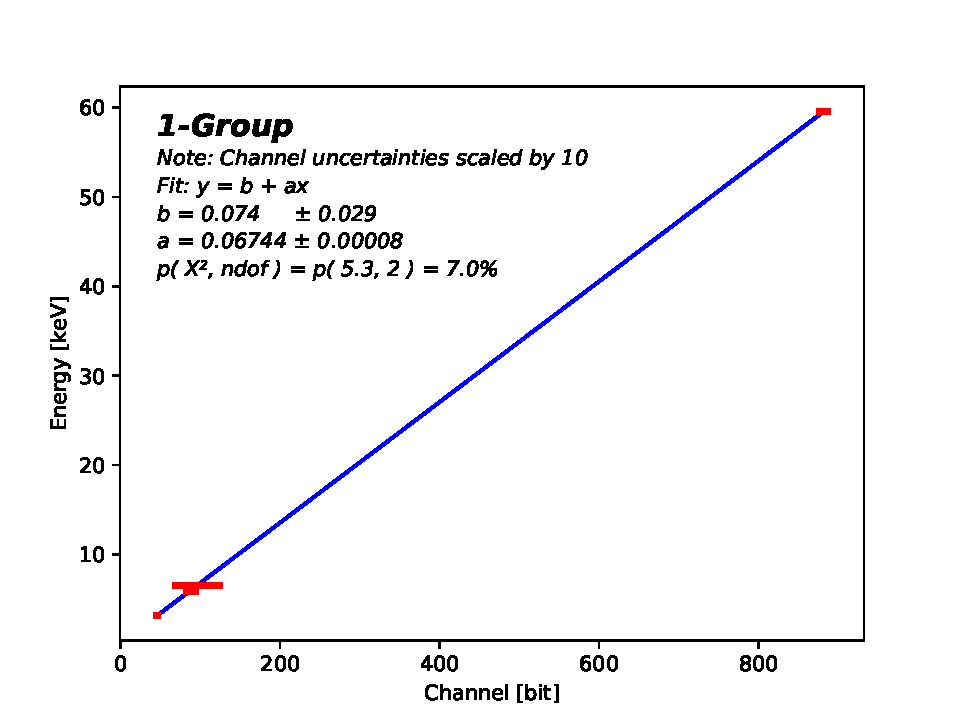
\includegraphics[width=0.49\textwidth,page=1]{graphics/energychannelcalib.pdf}
  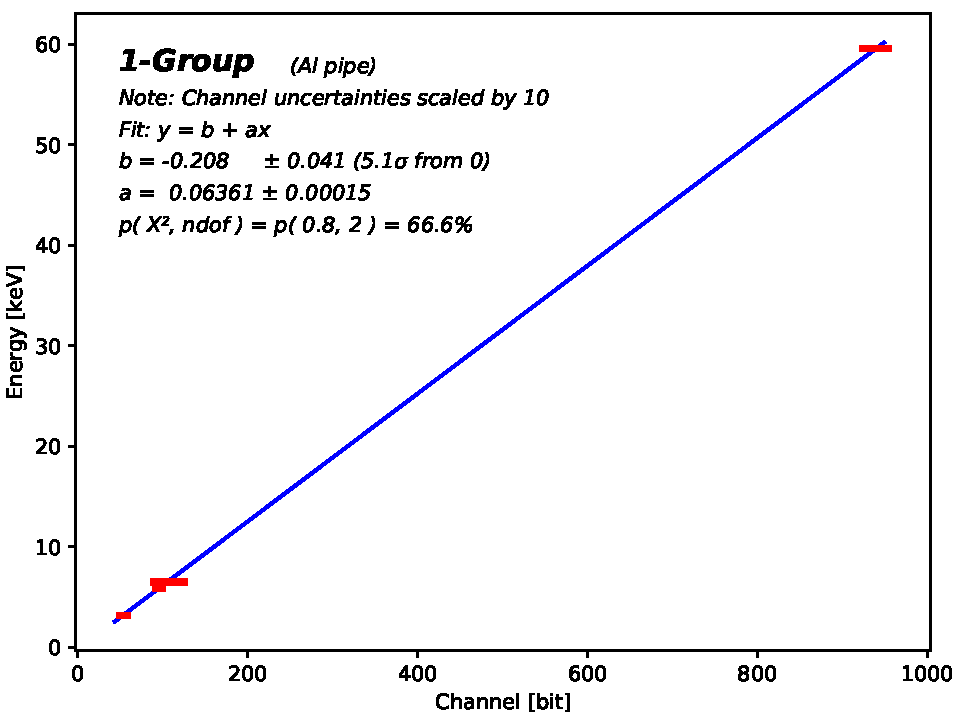
\includegraphics[width=0.49\textwidth,page=1]{graphics/aluenergychannelcalib.pdf}
  \caption{}
  \label{fig:energychannelcalib}
\end{figure*}

todo: \\
- table of all peaks and energies for can and alu \\
- final figure and the 4 gauss simultaneous fit for can \\
- comment on splitting uncertainties into stat. and calib. \\

%\subsection{Fe$^{55}$}

%\subsection{Am$^{81}$}
